\subsection{Recap: Quality Assurance}
\begin{frame}{Recap: Software Quality} % caution: slide copied from testing lecture
	\rightorleft{
		\mydefinition{Quality \mysource{\ludewiglichter}}{Quality is the entirety of properties and characteristics of a product or process that indicate adequacy with respect to given requirements.}
		\mydefinition{Quality Assurance \mysource{\ludewiglichter}}{Quality assurance \deutsch{Qualitätssicherung} are all activities with the goal to improve the quality.}
	}{
		\vspace{-12mm}
		\centering
		\pic[width=\linewidth,trim=0 240 0 300,clip]{andy-hunt}
		\vspace{-7mm}
		
		\mynote{Andy Hunt \mysource{\thepragmaticprogrammer}}{\mycite{No one in the brief history of computing has ever written a piece of perfect software. It's unlikely that you'll be the first.}}
		% co-authored The Pragmatic Programmer, known for the Agile Manifesto
	}
\end{frame}

\begin{frame}{Recap: Quality Assurance \mytitlesource{\ludewiglichter}} % caution: slide copied from testing lecture
	\hfill%
	\only<1|handout:0>{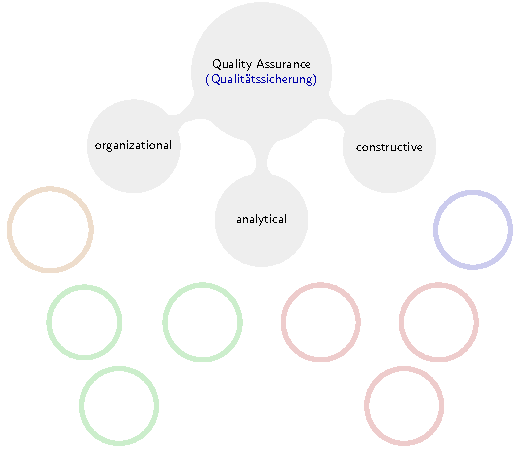
\includegraphics[height=\textheightwithtitle,page=1]{quality-assurance}}%
	\only<2|handout:0>{\includegraphics[height=\textheightwithtitle,page=2]{quality-assurance}}%
	\only<3|handout:0>{\includegraphics[height=\textheightwithtitle,page=3]{quality-assurance}}%
	\only<4|handout:0>{\includegraphics[height=\textheightwithtitle,page=4]{quality-assurance}}%
	\only<5|handout:1>{\includegraphics[height=\textheightwithtitle,page=5]{quality-assurance}}%
	\only<6|handout:0>{\includegraphics[height=\textheightwithtitle,page=6]{quality-assurance}}%
	% TODO check why this mindmap has a white background. could be large without a white background when using \textheightwithouttitle
\end{frame}

%mit nem emotionalen Bild motivieren => gute Softwarequalität ist wichtig

% mit quadranten starten
%bezug auf FM-analyse
%wir gucken uns jetzt Source Code an (evtl. linke zwei (VL 4, Problem Space) + rechte zwei Quadranten (VL 10+, Solution Space))
% wechselwirkung zw. sol und problem space (mapping+FM)

% properties one might want to analyze, similar to questions about feature models in modeling.tex
% include questions for all four quadrants

%zB Lego-Beispiel verwenden?

%strategien high-level angucken
%product-based
%number crunching, wie groß sind SPLs, product-based skaliert nicht

%ich könnte weniger produkte angucken (sampling)
%grundstein für test-vorlesung

%oder nur features angucken: feature-based
%wichtige message: es reicht nicht, features einzeln zu analysieren
%rückgriff auf interaktionen (dass feature-based nicht reicht)

%feature-product

%family (motivieren)

\subsection{Asking Questions About Product Lines}

\subsection{Classification of Product-Line Analyses (SPLE?)}

\subsection{Classification of Product-Line Analyses (CSUR? im 3. Block?)}

\subsection{Complexity of Product Lines}
\begin{frame}{\myframetitle}
	\leftorright{
		\mydefinition{Product-Line Complexity Classes}{
			In a timeframe of 24h \ldots
			\begin{enumerate}
				\item[\color{gray}\textbf{NC}] {\color{gray}Products cannot be generated automatically}
				\item[\textbf{C1}] All products can be generated and \emph{tested}
				\item[\textbf{C2}] Not C1, but all \emph{products} can be \emph{generated}
				\item[\textbf{C3}] Not C2, but all \emph{configurations} can be \emph{generated} (AllSAT)
				\item[\textbf{C4}] Not C3, but the \emph{number of valid configurations} can be computed (\ssat{})
				\item[\textbf{C5}] Not C4, but \emph{whether there is a valid configuration} can be computed (SAT)
				\item[\textbf{C6}] It cannot be computed whether there is a valid configuration
			\end{enumerate}
		}
	}{
		\myexample{Examples}{
			\begin{enumerate}
				\item[\color{gray}\textbf{NC}] {\color{gray}all product lines with custom development in application engineering\\(e.g., components and services with glue code, white-box frameworks)}
				\item[\textbf{C1}] $< 2{\small,}000$ products for 1 min per product
				\item[\textbf{C2}] $< 90{\small,}000$ products for 1 s per product
				\item[\textbf{C3}] $< 10^{13}$ configurations for 1 ns per configuration
				\item[\textbf{C4}] older versions of Linux/Automotive05
				\item[\textbf{C5}] newer versions of Linux/Automotive05\\(see \evaluatingsharpsatsolvers)
				\item[\textbf{C6}] No example known
			\end{enumerate}
		}
	}
\end{frame}
